\section{Implementation}
\label{sec:implementation}

The model described in \cref{sec:model} can be implemented as a \ac{WFST}.
In particular, the model can be decomposed in two transducers, one for each term.
The final model is given by the composition of the two transducer.

\subsection{First term: $\prod_{i=1}^n P(w_i | t_i)$}
The first transducer $\lambda_{word2concept}$ assigns the tag with the highest probability to each word.
The transducer has a single state $0$ with many self transitions.
For each unique pair $(w_i, t_j)$, a self transition $w_i \rightarrow t_j$ is added to the transducer.
The cost associated to the transitions is computed as the negative logarithm of the probability of the pair $P(w_i, t_j)$:
\begin{equation*}
    cost(w_i \rightarrow t_j) = -ln(P(w_i, t_j)).
\end{equation*}

In addition, we must take care of \ac{OOV} words, i.e. words that are never observed in the training data and thus not present in lexicon.
Since we can not make any assumption about the concepts probability for unknown words, we choose a uniform distribution.
Thus, we add one extra self transition $\langle unk \rangle \rightarrow t_j$ for each concept $t_j$, with cost:
\begin{equation*}
    cost(\langle unk \rangle \rightarrow t_j) = -ln \Big( \frac{1}{n_{concepts}} \Big),
\end{equation*}
where $\langle unk \rangle$ is a special token used for the \ac{OOV} words.

The model is implemented with Bash script that computes all counts, costs and transition for the transducer.
The lexicons are computed using \texttt{OpenGrm NGram}.
The transducer is compiled to the \texttt{FST} format using \texttt{OpenFst}.

\subsection{Second term: $\prod_{i=1}^n P(t_i | t_{i-1})$}
The second transducer $\lambda_{concept\_lm}$ is a language model for the concepts.
It takes as input a sequence of concepts and computes its probability given the predecessors and the observed training data.

A general problem with language models is data sparseness:
since the language has an underlying structure and the training data is limited, not all tuples $(t_i, ..., t_m)$ are observed.
As a consequence, most probabilities have value $0$, which makes the probability of most words sequences $0$ as well.

To solve this problem, we introduce smoothing:
the unseen tuples are assigned a small probability even though the real observed probability is $0$.
The probability of frequent tuples is slightly reduced to make the joint probability sum up to $1$.

Many different smoothing methods have been proposed in the literature.
A simple technique is the Laplace smoothing:
we add imaginary training data with all possible n-gram combinations, each of them with frequency $1$.
For instance, for the bigram case, we can compute the smoothed probability as:
\begin{equation*}
    P(t_i | t_{i-1}) = \frac{C(t_{i-1}, t_i) + 1}{C(t_{i-1}) + V},
\end{equation*}
where $V$ is the size of the vocabulary of pairs $(t_i | t_{i-1})$.
\cref{sec:performances} compares the performances of the model with different smoothing methods. 

Opposite to the first term, we do not need to take care of \ac{OOV} words, since the first transducer can produce only concepts in the concepts' lexicon.

\subsection{Concept tagging}
To compute the most probable sequence of tags, each sentence is first compiled to a \ac{FSA} $\lambda_{sentence}$.
For each word $w_i$, we define a state $i$ and a transition from state $i-1$ to state $i$ that translate word $w_i$ in itself.
The initial state is $0$, the final state is $n$, where $n$ is equal to the length of the sentence.
\cref{fig:fsa_sentence} shows an example.

\begin{figure}[h]
	\centering
	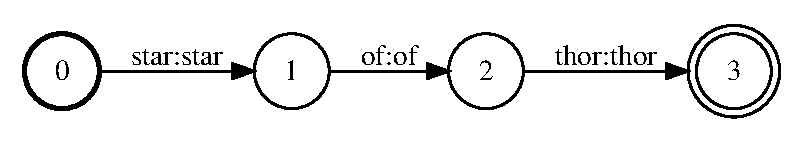
\includegraphics[width=.95\columnwidth]{figures/fsa}
	\caption{\ac{FSA} for the sentence ``star of thor''.}
	\label{fig:fsa_sentence}
\end{figure}

The most probable sequence of tags can be computed as the shortest path in the \ac{FST} given by the composition:
\begin{equation*}
    \lambda_{sentence} \circ \lambda_{word2concept} \circ \lambda_{concept\_lm}.
\end{equation*}
The shortest path is computed by the \texttt{OpenFst} library using the Viterbi algorithm.
This model is implemented in the file \texttt{model/v1.sh}.
